 \documentclass[11pt]{article}
\usepackage{geometry, titlesec}
\usepackage[parfill]{parskip}
\usepackage[italicdiff]{physics}
\usepackage{amsfonts, amsthm}
\usepackage[cm]{fullpage}
\usepackage{fancyhdr}
\usepackage{enumitem}
\usepackage{xcolor, soul}
\usepackage{kbordermatrix}
\usepackage{booktabs}
\usepackage{graphicx}
%\allowdisplaybreaks

\makeatletter
\renewcommand*\env@cases[1][1.2]{%
  \let\@ifnextchar\new@ifnextchar
  \left\lbrace
  \def\arraystretch{#1}%
  \array{@{}l@{\quad}l@{}}%
}
\makeatother

 
\renewcommand{\footrulewidth}{.2pt}
%\setlist[enumerate]{leftmargin=*}
\pagestyle{fancy}
\fancyhf{}
\lhead{\textbf{Physics 342 Homework 3}}
\rhead{Lacey Rainbolt}
\setlength{\headheight}{11pt}
\setlength{\headsep}{11pt}
\setlength{\footskip}{24pt}
\lfoot{\today}
\rfoot{\thepage}

\titleformat{\section}[runin]{\normalfont\large\bfseries}{Problem \thesection.}{1em}{}
\titleformat{\subsection}[runin]{\normalfont\large\bfseries}{\thesubsection}{1em}{}
\titleformat{\subparagraph}[leftmargin]{\normalfont\normalsize\bfseries}{}{0pt}{}

\newcommand{\refeq}[1]{(\ref{#1})}

\newcommand{\beq}{\begin{equation*}}
\newcommand{\eeq}{\end{equation*}}

\newcommand{\beqn}{\begin{equation}}
\newcommand{\eeqn}{\end{equation}}


\renewcommand{\vec}[1]{\mathbf{#1}}
\newcommand{\vfix}{\vspace{-\baselineskip}}


\newenvironment{statement}[1]
{
	\section{#1}
	\color{darkgray}
	\ignorespaces
}
{
%    \smallskip
}

\newenvironment{problem}
{
	\color{darkgray}
	\subsection{}
	\ignorespaces
}


\newenvironment{solution}
{
	\paragraph{Solution.}
}
{
	\bigskip
}

\newcommand{\Schrodinger}{Schr\"{o}dinger}
\newcommand{\qimplies}{\quad \implies \quad}


\begin{document}

\state{Spin-wave theory~(P\&S 11.1)}{\hfix}

\prob{ \label{1a}
	Prove the following wonderful formula: Let $\phix$ be a free scalar field with propagator $\ev{T \phix \phio} = \Dx$.  Then
	\eqn{show1}{
		\ev{ T e^{i \phix} e^{-i \phio} } = e^{[ \Dx - \Do ]}.
	}
	(The  factor $\Do$ gives a formally divergent adjustment of the overall normalization.)
}

\sol{
	According to P\&S~(9.18),
	\eq{
		\ev*{T \phi(\xq) \phi(\xw)}{\Omg} = \frac{\int \DDphi \phi(\xq) \phi(\xw) \exp[ i \int \ddqx \cL ]}{\int \DDphi \exp[ i \int \ddqx \cL ]}.
	}
	We use this expression to write the left-hand side of Eq.~\refeq{show1}:
	\eqn{thing1}{
		\ev{ T e^{i \phix} e^{-i \phio} } = \frac{\int \DDphi e^{i \phix} e^{-i \phio} \exp[ i \int \ddqy \cL ]}{\int \DDphi \exp[ i \int \ddqy \cL ]}
		= \frac{\int \DDphi \exp[i \phix - i \phio + i \int \ddqy \cL ]}{\int \DDphi \exp[ i \int \ddqy \cL ]}.
	}
	For a free Klein-Gordon~(i.e., scalar) field, Eq.~(9.39) tells us that the generating functional $\ZJ$ is given by
	\eq{
		\ZJ = \Zo \exp[ -\frac{1}{2} \int \ddqx \ddqy \Jx \DF(x - y) \Jy ],
	}
	where $\Zo = Z[0]$.  Thus, we want to find some $\Jy$ such that
	\eqn{thing1b}{
		\ev{ T e^{i \phix} e^{-i \phio} } = \frac{\ZJ}{\Zo}
	}
	where in general
	\eq{
		\ZJ = \int \DDphi \exp[ i \int \ddqx [ \cL + \Jx \phi(x) ] ]
	}
	by (9.34).  Inspecting Eq.~\refeq{thing1}, we recognize the denominator as $\Zo$ and see that if
	\eq{
		\Jy = \delq(y - x) - \delq(y)
	}
	we have an expression like Eq.~\refeq{thing1b}.  Collecting these findings, we have
	\al{
		\ans{ \ev{ T e^{i \phix} e^{-i \phio} } }&= \frac{\ZJ}{\Zo} \\
		&= \exp[ -\frac{1}{2} \int \ddqy \ddqz \Jy \DF(y - z) \Jz ] \\
		&= \exp[ -\frac{1}{2} \int \ddqy \ddqz \Jy \DF(y - z) [ \delq(z - x) - \delq(z) ] ] \\
		&= \exp[ -\frac{1}{2} \int \ddqy [ \delq(y - x) - \delq(y) ] [ \DF(y - x) - \DF(y) ] ] \\
		&= \exp[ -\frac{1}{2} [ \DF(0) - \DF(x) - \DF(-x) + \DF(0) ] ] \\
		&= \exp[ \DF(x) - \DF(0) ] \\
		&\ans{\; = e^{[ \Dx - \Do ]}, }
	}
	as we wanted to show. \qed
}



\prob{ \label{1b}
	We can use this formula in Euclidean field theory to discuss correlation functions in a theory with spontaneously broken symmetry for $T < \TC$.  Let us consider only the simplest case of a broken $O(2)$ or $U(1)$ symmetry.  We can write the local spin density as a complex variable
	\eq{
		\sx = \sqx + i \swx.
	}
	The global symmetry is the transformation
	\eq{
		\sx \to e^{-i \alp} \sx.
	}
	If we assume that the physics freezes the modulus of $\sx$, we can parameterize
	\eqn{sx}{
		\sx = A e^{i \phix}
	}
	and write an effective Lagrangian for the field $\phix$.  The symmetry of the theory becomes the translation symmetry
	\eqn{symmetry}{
		\phix \to \phix - \alp.
	}
	Show that (for $d > 0$) the most general renormalizable Lagrangian consistent with this symmetry is the free field theory
	\eqn{show1b}{
		\cL = \frac{1}{2} \rho(\vgrad \phi)^2.
	}
	In statistical mechanics, the constant $\rho$ is called the \emph{spin wave modulus}.  A reasonable hypothesis for $\rho$ is that it is finite for $T < \TC$ and tends to 0 as $T \to \TC$ from below.
}

\sol{
	In accordance with the Klein-Gordon Lagrangian in P\&S~(2.6),
	\eqn{KGL}{
		\cL_\text{K-G} = \frac{1}{2} (\pt \phi)^2 - \frac{1}{2} m^2 \phi^2,
	}
	we interpret $(\vgrad \phi)^2$ as $(\pt \phi)^2$.
	
	The Lagrangian cannot have terms of $\order{\phi^n}$ for any $n \neq 0$ since $\phi(x)$ is not invariant under Eq.~\refeq{symmetry}.  Any combination of derivatives of $\phi$ is invariant, however, since $\alp$ is a constant and does not contribute to any derivative.  Thus, only terms like $\pt^n \phi^m$ (where $n$ denotes a power of $\pt$) for $n, m > 0$ and $n \geq m$ are consistent with the symmetry of Eq.~\refeq{symmetry} for $d$ an integer.
	
	Now we must determine which of these terms are renormalizable.  We know that the Lagrangian must have dimension $d$, and that $\phi$ has dimension $(d - 2) / 2$.  Taking a derivative adds a mass dimension.  The theory is renormalizable if the coupling constant $\rho$ has dimension greater than or equal to 0~\cite[p.~322]{Peskin}.  Let $p$ be the dimension of $\rho$.  The dimension of our allowed term is then
	\eq{
		[ \rho \pt^n \phi^m ] = p + n + m \frac{d - 2}{2},
	}
	which we require to be equal to $d$.  Thus we seek solutions to the system of equations
	\al{
		d &= p + n + m \frac{d - 2}{2}, &
		n &\geq m, &
		p &\geq 0.
	}
	Solving with Mathematica, we find that this system has two solutions: $n = m = 2$ and $p = 0$; and $n = m = 1$ and $p = d / 2$.  However, the term $\pt \phi$ for $n = m = 1$ does not contribute to the action because it is a total derivative and does not contribute when the integral over $\cL$ is evaluated:
	\eq{
		\int \dd[d]{x} \pt\phi = \phi \bigg|_{-\infty}^\infty
		= 0.
	}
	Thus the only possibility is $n = m = 2$.  Note that
	\eq{
		\pt^2 \phi^2 = \pt(\pt \phi^2)
		= 2 \pt( \phi \pt \phi)
		= \pt \phi \pt \phi + \phi \pt^2 \phi
		= (\pt \phi)^2,
	}
	since $\phi \pt^2 \phi$ is not invariant under Eq.~\refeq{sx}.  This means that $\rho$ must be dimensionless and that the only allowed terms in the Lagrangian are proportional to $(\pt \phi)^2$, which is consistent with Eq.~\refeq{show1b}. \qed
}



\prob{
	Compute the correlation function $\ev{ \sx \sao }$.  Adjust $A$ to give a physically sensible normalization (assuming that the system has a physical cutoff at the scale of one atomic spacing) and display the dependence of this correlation function on $x$ for $d = 1, 2, 3, 4$.  Explain the significance of your results.
}

\sol{
	Applying Eq.~\refeq{sx},
	\eq{
		\ev{ \sx \sao } = \ev*{ A e^{i \phix} \As e^{-i \phio} }
		= \ev*{ \abs{A}^2 } \ev*{ e^{i \phix} e^{-i \phio} }.
	}
	Now we can apply Eq.~\refeq{show1} to find
	\eqn{thing1c}{
		\ans{ \ev{ \sx \sao } = \abs{A}^2 \exp[ D(x) - D(0) ], }
	}
	where $D(x - y)$ is a Green's function.  Since our Lagrangian is similar to the Klein-Gordon Lagrangian Eq.~\refeq{2.6}, our Green's function is similar to that of the Klein-Gordon operator, which is given by P\&S~(2.56):
	\eq{
		(\pt^2 + m^2) D(x - y) = -i \delq(x - y).
	}
	The Feynman prescription for this Green's function is given by (2.59),
	\eqn{DF}{
		\DF(x - y) = \int \ddqpf \frac{i}{p^2 - m^2 + i \eps} e^{-i p \cdot (x - y)}.
	}
	For the Lagrangian in Eq.~\refeq{show1b}, we set $m = 0$ and insert a factor of $\rho$:
	\eq{
		\rho \pt^2 D(x - y) = -i \deld(x - y),
	}
	so adapting Eq.~\refeq{DF} for this situation yields
	\eqn{DF}{
		\DF(x - y) = \frac{1}{\rho} \int \dddpf \frac{i}{p^2 + i \eps} e^{-i p \cdot (x - y)}.
	}
	We see that $\DF(0)$ diverges, so we absorb it into the constant to make the normalization physically sensible.  We can do this because, as we showed in \ref{1b}, the theory is renormalizable.  Define $A'$ such that
	\eq{
		{A'}^2 = \abs{A}^2 e^{-D(0)}.
	}
	Then Eq.~\refeq{thing1c} can be written
	\eq{
		\ans{ \ev{ \sx \sao } =  {A'}^2 e^{D(x)}. }
	}
	
	To evaluate the divergent integral $D(x)$, we look to the Feynman parameter method we have been using to solve divergent integrals.  Apparently, the Schwinger parametrization is useful in deriving the Feynman parametrization, and it is given by~\cite{Feynman}
	\eq{
		\frac{1}{A} = \intoi \dds e^{-s A}.
	}
	Using this equation, we can write Eq.~\refeq{DF} as
	\eq{
		\DF(x) = \frac{1}{\rho} \int \dddpf \frac{i}{p^2} e^{-i p \cdot x}
		= \frac{i}{\rho} \int \dddpf \intoi \dds e^{-s p^2} e^{-i p \cdot x}.
	}
	Now we can complete the square in the exponential to get a Gaussian integral:
	\al{
		\DF(x) &= \frac{i}{\rho} \int \dddpf \intoi \dds \exp[ -s p^2 - i p \cdot x + \frac{x^2}{4 s} - \frac{x^2}{4 s} ] \\
		&= \frac{i}{\rho} \int \dddpf \intoi \dds \exp[ -s \paren{ p + \frac{i x}{2 s} }^2 - \frac{x^2}{4 s} ] \\
		&= \frac{i}{\rho (2 \pi)^d} \intoi \dds e^{-x^2 / 4 s} \int \dd[d]{u} e^{-s u^2} \\
		&= \frac{i}{\rho (2 \pi)^{d}} \intoi \dds e^{-x^2 / 4 s} \sqrt{ \frac{(2\pi)^d}{(2s)^d} } \\
		&= \frac{i}{\rho (4 \pi)^{d / 2}} \intoi \dds \frac{e^{-x^2 / 4 s}}{s^{d / 2}}
	}
	where we have used~\cite{QFT}
	\eq{
		\int \exp( -\frac{1}{2} x \cdot A \cdot x ) \dd[n]{x} = \sqrt{\frac{(2\pi)^n}{\det A}},
	}
	with $A$ a $d \times d$ diagonal matrix $2s$.  Using Mathematica to integrate with respect to $s$, we find
	\eq{
		\DF(x) = \frac{i}{\rho (4 \pi)^{d / 2}} \frac{2^{d - 2}}{x^{d - 2}} \Gam(d / 2 - 1)
		= \frac{i}{4 \pi^d \rho} \Gam(d / 2 - 1) x^{2 - d}.
	}
	The gamma function diverges as $d \to 2$, so as we have done in previous problems, we expand about $\eps = 2 - d$.  Evaluating the series expansion using Mathematica, we obtain
	\eq{
		\DF(x) = \frac{i}{4 \pi^{1 - \eps} \rho} \Gam(\eps / 2) x^\eps
		\approx \frac{i}{4 \pi \rho} \paren{ \frac{2}{\eps} - \gam + 2 \ln(\pi x) }
		\sim \frac{i}{2 \pi \rho} \ln(x)
		= i \ln(\frac{1}{x^{2 \pi \rho}}).
	}
	We Wick rotate $x \to i x$.  Then the dependence of the correlation function on $x$ for $d = 1, 2, 3, 4$ is
	\ans{\al{
		(d = 1) &\qquad \ev{ \sx \sao } \sim e^{-x / 2 \sqrt{\pi} \rho}, &
		(d = 2) &\qquad \ev{ \sx \sao } \sim x^{2 \pi \rho}, \\
		(d = 3) &\qquad \ev{ \sx \sao } \sim \frac{1}{x}, &
		(d = 4) &\qquad \ev{ \sx \sao } \sim \frac{1}{x^2}.
	}}%
	In $d > 2$ dimensions, the expectation value of the correlation function tends to 0 at large distances $x$.  For $d > 2$, it drops off more quickly as $d$ increases.  The $d \leq 2$ cases depend on $\rho$, which we assume is positive.  The $d = 1$ case drops off with increasing distance, and more quickly with smaller $\rho$.  For $d = 2$, the expectation value of the correlation function increases with increasing distance, and it blows up more quickly with larger $\rho$.
	
	These results are consistent with the Mermin--Wagner theorem, which states that a continuous symmetry cannot be broken in $d \leq 2$ dimensions~\cite{CMW}.  That is, in $d \leq 2$ dimensions, a symmetry-breaking field cannot have a nonzero vacuum expectation value~\cite[p.~460]{Peskin}.  A physical explanation is that each spin has more nearest neighbors in higher dimensions.  Since the spins are inclined to align with their neighbors, there is a higher degree of correlation in higher dimensions at the same distance.  In two dimensions, the correlations are weak enough that they are overpowered by the field fluctuations.
}



\newcommand{\Vo}{V_0}
\newcommand{\vr}{\vb{r}}
\newcommand{\Rl}{R_l}
\newcommand{\Ylm}{Y_{l m}}
\newcommand{\Rlr}{\Rl(r)}
\newcommand{\vep}{\varepsilon}
%\newcommand{\tht}{\theta}
\newcommand{\del}{\delta}
\newcommand{\dell}{\del_l}
\newcommand{\delo}{\del_0}
\newcommand{\Al}{A_l}
\newcommand{\absr}{\abs{r}}

\newcommand{\tsc}{\text{sc}}
\newcommand{\asc}{a_\tsc}
\newcommand{\kap}{\kappa}
\newcommand{\avep}{\abs{\vep}}

\newcommand{\betal}{\beta_l}
\newcommand{\psiE}{\psi_E}
\newcommand{\uE}{u_E}
\newcommand{\El}{E_l}
\newcommand{\eff}{\text{eff}}
\newcommand{\Veff}{V_\eff}

\newcommand{\jl}{j_l}
\newcommand{\jo}{j_0}
\newcommand{\nl}{n_l}
\newcommand{\hlq}{h_l^{(1)}}
\newcommand{\hoq}{h_0^{(1)}}
\newcommand{\Ro}{R_0}
\newcommand{\constant}{\text{constant }}


\clearpage
\begin{statement}{}
	Consider a quantum particle with mass $m$ moving in the presence of the square well potential
	\beq
		V(r) = \begin{cases}
			-\Vo & r \leq a, \\
			0 & r > a.
		\end{cases}
	\eeq
	\vfix
\end{statement}

\begin{problem}
	Writing the wave function in polar coordinates as $\psi(\vr) = \Rlr \, \Ylm(\tht, \phi)$, write down the {\Schrodinger} equation obeyed by $\Rl$.
\end{problem}

\begin{solution}
	From (A.5.1) in Sakurai, the full {\Schrodinger} equation is
	\beq
		-\frac{\hbar^2}{2m} \left[ \frac{1}{r^2} \pdv{r} \left( r^2 \pdv{\psiE}{r} \right) + \frac{1}{r^2 \sin\tht} \pdv{\tht} \left( \sin\tht \pdv{\psiE}{\tht} \right) + \frac{1}{r^2 \sin^2\tht} \pdv[2]{\psiE}{\phi} \right] + V(r) \,\psiE = E \psiE,
	\eeq
	where the angular part of $\psiE$ satisfies (A.5.4),
	\beq
		-\left[ \frac{1}{\sin\tht} \pdv{}{\tht} \left( \sin\tht \pdv{}{\tht} \right) + \frac{1}{\sin^2\tht} \pdv[2]{}{\phi} \right] \Ylm = l (l + 1) \Ylm.
	\eeq
	Then the equivalent one-dimensional {\Schrodinger} equation is the equation immediately following (A.5.8),
	\beqn \label{schrod}
		-\frac{\hbar^2}{2m} \dv[2]{\uE}{r} + \left[ V(r) + \frac{l (l + 1) \hbar^2}{2 m r^2} \right] \uE = E \uE,
	\eeqn
	where $\uE(r) = r R(r)$.  In terms of $\Rl$,
	\beq
		-\frac{\hbar^2}{2m} \dv[2]{r} (r \Rl) + \left[ V(r) + \frac{l (l + 1) \hbar^2}{2 m r^2} \right] r \Rl = E r \Rl.
	\eeq
	or
	\beq
		\frac{\hbar^2}{2 m} \left[ -\frac{1}{r^2} \pdv{r} \left( r^2 \pdv{r} \right) + V(r) + \frac{l (l + 1)}{r^2} \right] \Rl(r) = \El \, \Rl(r).
	\eeq
	From (7.7.1), the effective potential at low energies for the $l$th partial wave is
	\beq
		\Veff = V(r) + \frac{\hbar^2}{2m} \frac{l (l + 1)}{r^2},
	\eeq
	so the {\Schrodinger} equation can be rewritten as
	\beq
		\left[ -\frac{\hbar^2}{2 m} \frac{1}{r^2} \pdv{}{r} \left( r^2 \pdv{}{r} \right) + \Veff\, \right] \Rl(r) = \El \, \Rl(r).
	\eeq
	\vfix
\end{solution}

\begin{problem}
	When $\Vo$ is a certain value, there is one bound state for the $s$ wave ($l = 0$).  The bound state energy $\vep$ is small ($0 < \avep \ll \Vo$).  Obtain the range of the depth of the well $\Vo$ (? $\leq \Vo <$ ?).  Also, calculate for the bound state the probability for the particle to exist outside of the well.
\end{problem}

\begin{solution}
	Inside the well, $\Rl$ are given by (A.5.16),
	\beq
		\Rl(r) = \constant \jl(\alp r),
	\eeq
	where $\alp$ is defined in Eq.~(A.5.17),
	\beq
		\alp = \sqrt{\frac{2m (\Vo - \abs{E})}{\hbar^2}}, \quad r < a,
	\eeq
	and the spherical Bessel functions $\jl$ is given by (A.5.12),
	\begin{align*}
		\jl(\rho) = \sqrt{\frac{\pi}{2\rho}} J_{l + 1/2}(\rho).
	\end{align*}
	For the $s$ wave, the relevant Bessel function is given by (A.5.12),
	\beq
		\jo(\rho) = \frac{\sin\rho}{\rho}.
	\eeq
%	Then we have
%	\beqn \label{inside}
%		\Ro(r) \propto \sqrt{\frac{\hbar^2}{2 m (\Vo - \avep)}} \frac{1}{r} \sin(\sqrt{\frac{2 m \Vo}{\hbar^2}} r), \quad r < a,
%	\eeqn
%	for the solution inside the well.
	But for $l - 0$, $\Veff$ reduces to $V(r)$, so \refeq{schrod} reduces to the one-dimensional problem for $\uE$,
	\beq
		-\frac{\hbar^2}{2m} \dv[2]{\uE}{r} + V(r) \uE = E \uE.
	\eeq
	The bound-state solutions are given by (A.2.6),
	\beq
		\uE \sim \begin{cases}
			e^{-\kap r} & \text{for } r > a, \\
			\cos kr \quad \text{(even parity)} & \text{for } r < a, \\
			\sin kr \quad \text{(odd parity)} & \text{for } r > a,
		\end{cases}
	\eeq
	where $k$ and $\kap$ are defined by (A.2.7),
	\begin{align*}
		k &= \sqrt{\frac{2m (\Vo - \abs{E})}{\hbar^2}}, &
		\kap &= \sqrt{\frac{2m \abs{E}}{\hbar^2}}.
	\end{align*}
	So we see that $\alp = k$, and thus we are interested in the odd-parity solutions to the one-dimensional problem.
	
	For the one-dimensional problem, the allowed values of bound-state energy
	\beq
		E = -\frac{\hbar^2 \kap^2}{2m}
	\eeq
	can be found by solving (A.2.8),
	\begin{align*}
		k a \tan k a &= \kap a \quad\text{(even parity)}, &
		k a \cot k a &= -\kap a \quad\text{(odd parity)},
	\end{align*}
	where $\kap$ and $k$ are related by (A.2.9),
	\beq
		\frac{2 m \Vo a^2}{\hbar^2} = (k^2 + \kap^2) a^2.
	\eeq
	We are interested in the odd parity solutions, so we want to solve
	\beqn \label{ka}
		k a \cot k a = -\kap a.
	\eeqn
	For the right side, we can write
	\beqn \label{kapa}
		\kap a = -\sqrt{\frac{2 m \Vo a^2}{\hbar^2} - k^2 a^2} \equiv -\sqrt{z^2 - (ka)^2},
	\eeqn
	where we have defined $z$.
	
	Now we can solve the equation graphically.  Note that $ka$ and $z$ are both positive definite. This means the odd parity equation in \refeq{ka} has its first $ka$ axis intercept at $ka = \pi/2$, where the slope is negative.  Note also that $\kap a$ given by \refeq{kapa} is an equation for one quarter of an ellipse in quadrant IV, so it is not defined above the $ka$ axis.  Therefore it is not possible for the two graphs to intersect for $z < \pi / 2$.  For $z > 3\pi / 2$, the plots intersect twice, meaning there is more than one bound state.  In Fig.~\ref{plot}, this is illustrated with $\kap a$ for $z = n \pi / 2$ with $n = 1, 2, 3, \ldots$.
	
	\begin{figure} \centering
		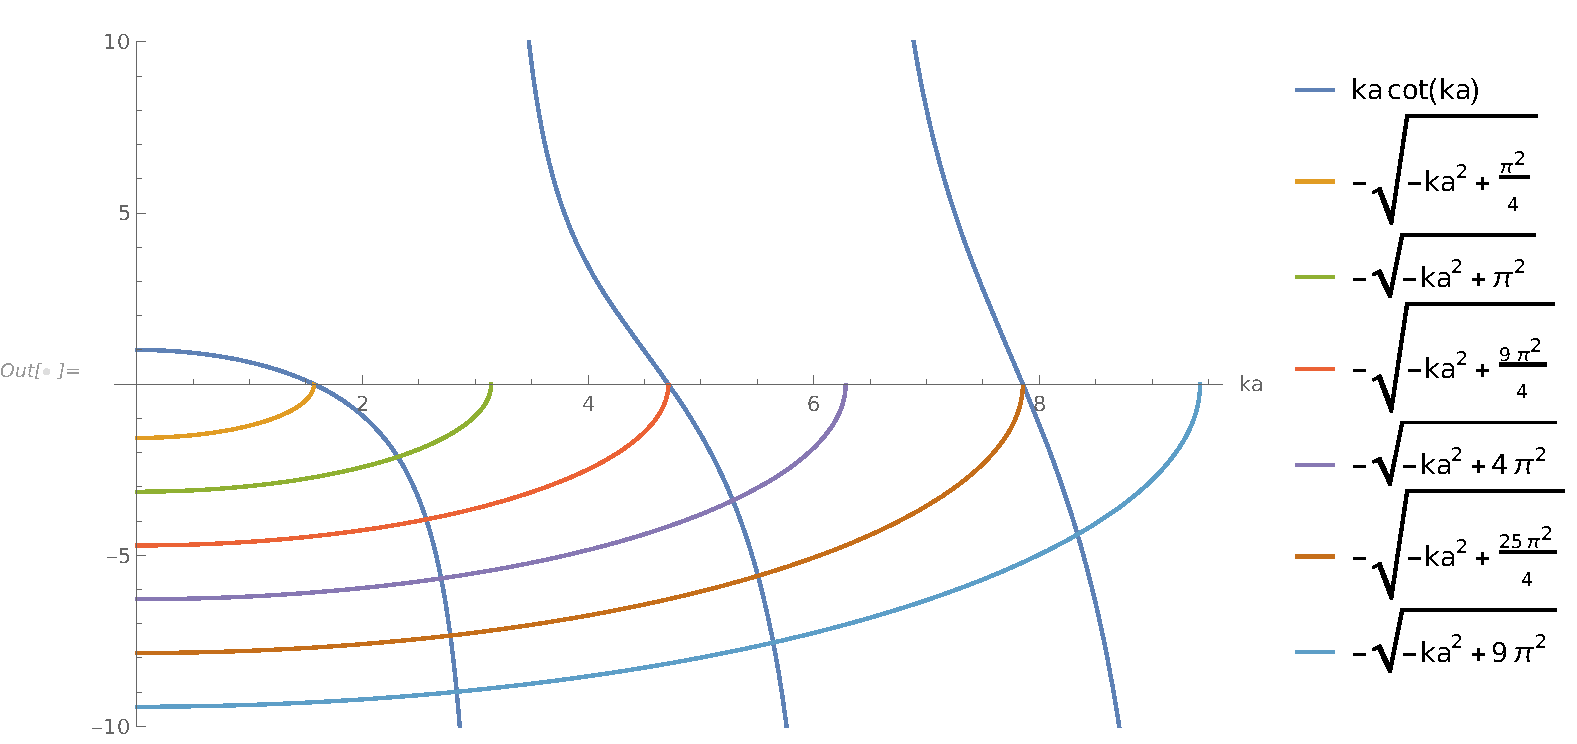
\includegraphics[trim=2cm 0 0 0,clip,width=0.75\textwidth]{plot}
		\caption{Plot demonstrating single bound state solutions to \refeq{ka} in the range $\pi/2 < z < 3\pi/2$, where $z$ is defined in \refeq{kapa}.}
		\label{plot}
	\end{figure}
	
	Finally, we have the restriction
	\beq
		\frac{\pi}{2} < \sqrt{\frac{2 m \Vo a^2}{\hbar^2}} < \frac{3\pi}{2}
		\qimplies
		\frac{\pi^2 \hbar^2}{8 m a^2} < \Vo < \frac{9\pi^2 \hbar^2}{8 m a^2}.
	\eeq
	\vfix
\end{solution}



\begin{problem}
	Consider the scattering problem by the well.  For each $l$, for large enough $r$, when $\Rlr$ is given by $\Rlr \sim \Al \sin(kr - l\pi / 2 + \dell) / r$, $\dell$ is called the scattering phase shift.  For the value of $\Vo$ within the range you obtained in the above problem, when the energy of the incident wave is is $E = 9 \Vo / 16$, calculate $\tan\delo$~(where $\delo$ is the scattering phase shift for the $s$ wave).
\end{problem}

\begin{solution}
%	From (7.6.35) in Sakurai,
%	\beq
%		\tan\dell = \frac{k R \jl'(kR) - \betal \jl(kR)}{k R \nl'(kR) - \betal \nl(kR)},
%	\eeq
%	where (7.6.34) defines $\betal$,
%	\beq
%		\betal \equiv \left[ \frac{r}{\Al} \dv{\Al}{r} \right]_{r=R},
%	\eeq
%	and
%	\beq
%		\jl'(kR) = \left. \dv{\jl}{(kr)} \right|_{kr = kR}
%	\eeq
\end{solution}

\begin{problem}
	Now consider the $S$ matrix, $S \equiv \exp(2i \delo) = \exp(i \delo) / \exp(-i \delo)$.  Compare the condition on $s$ wave bound state energies and the zero of the denominator of $S$.  Explain their relation.
\end{problem}




\newcommand{\gam}{\gamma}
\newcommand{\chio}{\chi_0}
\newcommand{\chior}{\chio(r)}
\newcommand{\Gam}{\Gamma}

\begin{statement}{}
	Consider a three dimensional potential
	\beq
		V(\absr) = \frac{\hbar^2 \gam}{2m} \del(\absr - a).
	\eeq
	The $s$ wave {\Schrodinger} equation is given by
	\beq
		-\frac{\hbar^2}{2m} \dv[2]{\chior}{r} + \frac{\hbar^2 \gam}{2m} \del(r - a) \, \chior = E \,\chior.
	\eeq
	The $s$ wave function must be regular (zero) at $r = 0$.  At $r = a$, it is continuous, but its derivative can jump.
\end{statement}

\begin{problem}
	Calculate the $s$ wave scattering phase shift $\do(k)$, where $k$ is related to $E$ as $E = \hbar^2 k^2 / 2m$.
\end{problem}

\begin{problem}
	When $\gam \gg k$, $1/a$ and when $\sin ka$ is not small, discuss the behavior of the scattering phase shift.
\end{problem}

\begin{problem}
	Obtain the condition to have resonant states and calculate the energy of the resonant states.
\end{problem}

\begin{problem}
	Calculate the width $\Gam$ of the resonance.  Discuss its behavior when $\gam$ is big.
\end{problem}

\begin{problem}
	When the velocity of the incident wave is small, obtain the scattering cross section.
\end{problem}



\vfill
I consulted Sakurai's \emph{Modern Quantum Mechanics}, Shankar's \emph{Principles of Quantum Mechanics}, and the Wikipedia article on a particle in a spherically symmetric potential while writing up these solutions.

\end{document}